\chapter{Variabel, Konstanta, Tipe Data Dasar, dan Konversi Tipe Data}

\section{Variabel}

Variabel merupakan tempat penyimpanan sementara yang digunakan untuk menampung data selama program berjalan, sehingga data tersebut dapat digunakan kembali. Berbeda dengan bahasa pemrograman \textit{static type} seperti C, C++, dan Java yang harus secara eksplisit menulis tipe data untuk variabel. Di Python, variabel memiliki tipe data yang dinamis (\textit{dynamic type}) dan dapat berubah sesuai dengan kebutuhan program.
\newline

\begin{figure}[H]
	\centering
	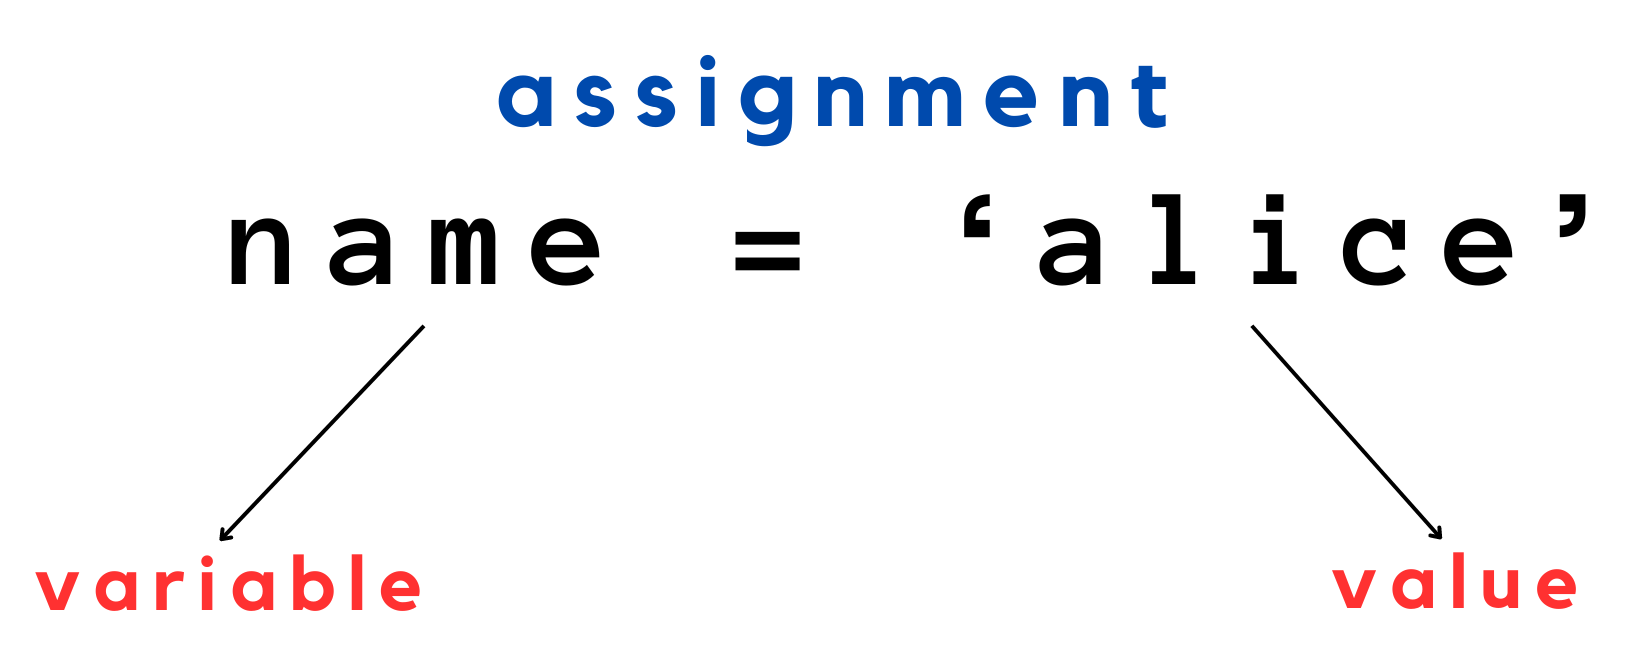
\includegraphics[width=0.7\textwidth]{../shared_assets/images/python_variable_structure.png}
	\caption{Struktur Variabel di Python}
	\label{fig:python-variable-structure}
\end{figure}

\noindent
Sumber gambar: \url{https://www.packetswitch.co.uk/python-variables-data-types/}

\subsection{Aturan Penamaan Variabel}

Pemberian nama variabel di Python harus mematuhi beberapa aturan penamaan yang disediakan oleh Python. Berikut adalah beberapa aturan penamaan variabel di Python:

\begin{itemize}
	\item Nama variabel harus dimulai dengan huruf atau underscore (\_).
	\item Nama variabel tidak boleh dimulai dengan angka.
	\item Nama variabel tidak boleh mengandung spasi.
	\item Nama variabel tidak boleh mengandung simbol.
	\item Nama variabel tidak boleh mengandung kata kunci (\textit{keyword}) yang sudah terdefinisi dalam Python, seperti \texttt{def}, \texttt{for}, \texttt{if}, \texttt{return}, dan sebagainya.
\end{itemize}

\subsection{Latihan Membuat Variabel}

Buat file baru dengan nama \textbf{variable.py} dan buat variabel dengan nama \textbf{nama}, \textbf{usia}, dan \textbf{berat_badan} dengan tipe data yang sesuai dan nilai-nilai yang sesuai. Kemudian cetak variabel tersebut.

\begin{lstlisting}[style=PythonStyle, caption={Kode Python: variable.py}]
nama = "Stefani Laurensia"
usia = 21
berat_badan = 50.2

print(nama)
print(usia)
print(berat_badan)
\end{lstlisting}

\subsection{Contoh Kesalahan Penamaan Variabel}

\begin{lstlisting}[style=PythonStyle, caption={Kode Python: variable.py}]
1angka = 200 # Nama variabel tidak boleh dimulai dengan angka
nama lengkap = "Budi" # Nama variabel tidak boleh mengandung spasi
gaji$ = 1000000 # Nama variabel tidak boleh mengandung simbol
class = "Informatika" # class merupakan kata kunci untuk membuat sebuah class di Python sehingga melanggar aturan di mana nama variabel tidak boleh mengandung kata kunci
\end{lstlisting}

\section{Konstanta}

Konstanta adalah variabel yang seharusnya nilainya tidak berubah selama program berjalan. Contohnya nilai \textbf{\textit{pi}} (3.14) atau gravitasi (9.81). Di Python, kita bisa menandai variabel sebagai Final dari modul \texttt{typing} untuk memberi tanda bahwa variabel tersebut dimaksudkan sebagai konstanta. Namun ada hal-hal yang perlu diperhatikan:
\begin{itemize}
	\item Python tidak memaksa variabel \texttt{Final} agar tidak bisa diubah.
	\item Penandaan \texttt{Final} hanya \textbf{memberi peringatan pada type checker}, bukan mencegah perubahan di runtime.
\end{itemize}

\subsection{Aturan Penamaan Konstanta}

Untuk menandakan bahwa sebuah variabel adalah konstanta, kita bisa menggunakan huruf besar untuk membedakan dengan variabel biasa. Hal ini mengikuti aturan penamaan variabel yang dibuat oleh Python (\href{https://peps.python.org/pep-0008/}{PEP 8 - Style Guide for Python Code}).

\subsection{Latihan Membuat Konstanta}

Buat file baru dengan nama \textbf{constant.py} dan buat konstanta dengan nama \textbf{PI} dan \textbf{GRAVITASI} dengan nilai yang sesuai. Kemudian cetak konstanta tersebut. Namun, berbeda dari bahasa pemrograman lain seperti C, C++, atau Java, di Python konstanta dapat diubah.
\begin{lstlisting}[style=PythonStyle, caption={Kode Python: constant.py}]
from typing import Final

PI: Final = 3.14
GRAVITASI: Final = 9.81

print(PI)
print(GRAVITASI)

GRAVITASI = 10 # Nilai masih tetap bisa berubah, tapi tidak disarankan
print(GRAVITASI)
\end{lstlisting}

\section{Tipe Data Dasar}

Tipe data merupakan jenis data yang bisa disimpan di program Python. Tipe data di Python memiliki banyak jenis, seperti \texttt{int}, \texttt{float}, \texttt{str}, \texttt{bool}, \texttt{list}, \texttt{tuple}, \texttt{dict}, dan \texttt{set}. Namun pada \textit{chapter} kali ini, kita akan fokus pada tipe data dasar, antara lain \texttt{int}, \texttt{float}, \texttt{str}, dan \texttt{bool}.
\newline \newline
Berdasarkan kelompoknya, tipe data dasar di Python dapat dibedakan menjadi 3 kelompok, antara lain:

\begin{enumerate}
\item \textbf{Numeric} (Angka)
\begin{enumerate}
\item \textbf{Integer} (bilangan bulat)
\begin{lstlisting}[style=PythonStyle]
usia = 18
jumlah_mahasiswa = 64
nomor_rumah = 88

suhu = -5
\end{lstlisting}

\item \textbf{Float} (bilangan desimal)
\begin{lstlisting}[style=PythonStyle]
koordinat_x = 5.5
koordinat_y = 7.8

saldo = 10.500.075
\end{lstlisting}
\end{enumerate}

\item \textbf{Teks} (Kata / Kalimat)
\begin{enumerate}
\item \textbf{String} (kumpulan karakter)
\begin{lstlisting}[style=PythonStyle]
nama = "John"
quote = 'Programmer: A machine that turns coffee into code'
pesan_email = """
Kepada Yth. John Doe,

Terima kasih atas pesanan anda.
"""
\end{lstlisting}
\end{enumerate}

\item \textbf{Boolean} (Benar atau Salah)
\begin{lstlisting}[style=PythonStyle]
is_married = False
is_single = True
\end{lstlisting}
\end{enumerate}

\section{Konversi Tipe Data (\textit{Type Casting})}

Kadang kita perlu mengubah tipe data dari satu jenis ke jenis lain agar Python bisa memprosesnya dengan benar.
Misal, input dari pengguna melalui fungsi \texttt{input()} selalu mengembalikan tipe data string (str), tapi kita ingin melakukan perhitungan angka, maka kita harus mengubahnya menjadi int atau float.

\begin{table}[h!]
\centering
\begin{tabular}{|c|c|c|}
\hline
\textbf{Fungsi} & \textbf{Keterangan} & \textbf{Contoh} \\
\hline
int() & Ubah menjadi bilangan bulat & int("10") → 10 \\
\hline
float() & Ubah menjadi bilangan desimal & float("3.14") → 3.14 \\
\hline
str() & Ubah menjadi teks & str(10) → "10" \\
\hline
bool() & Ubah menjadi True/False & bool(0) → False, bool(5) → True \\
\hline
\end{tabular}
\caption{Fungsi Untuk Konversi Tipe Data di Python}
\end{table}

\subsection{Latihan Konversi Tipe Data}

\begin{lstlisting}[style=PythonStyle, caption={Kode Python: string_to_int.py}]
usia = input("Masukkan usia Anda: ")
print("Tipe data sebelum konversi:", type(usia)) # Menampilkan tipe data sebelum konversi

usia = int(usia) # Konversi tipe data string menjadi integer
print("Tipe data setelah konversi:", type(usia)) # Menampilkan tipe data setelah konversi

usia_lima_tahun_kemudian = usia + 5 # Perhitungan usia 5 tahun kemudian
print("Usia 5 tahun kemudian:", usia_lima_tahun_kemudian)
\end{lstlisting}

\begin{lstlisting}[style=PythonStyle, caption={Kode Python: string_to_float.py}]
angka_str = "45.67"
print("Sebelum konversi:", angka_str, type(angka_str))

angka_float = float(angka_str)
print("Setelah konversi ke float:", angka_float, type(angka_float))
\end{lstlisting}

\begin{lstlisting}[style=PythonStyle, caption={Kode Python: int_to_float.py}]
angka_int = 10
print("Sebelum konversi:", angka_int, type(angka_int))

angka_float = float(angka_int)
print("Setelah konversi ke float:", angka_float, type(angka_float))
\end{lstlisting}

\begin{lstlisting}[style=PythonStyle, caption={Kode Python: float_to_int.py}]
angka_float = 3.99
print("Sebelum konversi:", angka_float, type(angka_float))

angka_int = int(angka_float)
print("Setelah konversi ke integer:", angka_int, type(angka_int))
\end{lstlisting}

\subsection{Kesalahan dalam Konversi Tipe Data}
Meskipun Python menyediakan fungsi bawaan untuk mengubah tipe data (\texttt{int()}, \texttt{float()}, \texttt{str()}, \texttt{bool()}), \textbf{tidak semua konversi bisa dilakukan dengan sukses}. Jika nilai yang dikonversi tidak sesuai dengan tipe data tujuan, maka program akan menghasilkan \textbf{error}. Berikut adalah contoh kesalahan dalam konversi tipe data:

\begin{lstlisting}[style=PythonStyle]
# String huruf → Integer
huruf = "abc"
huruf_integer = int(huruf) 
# Output: ValueError: invalid literal for int() with base 10: 'abc'

# String bilangan desimal → Integer
angka_str = "12.34"
angka_int = int(angka_str)  
# Output: ValueError: invalid literal for int() with base 10: '12.34'
\end{lstlisting}

Perhatikan pada contoh di atas bahwa program akan menghasilkan \textbf{error} ketika nilai yang dikonversi tidak sesuai dengan tipe data tujuan. Hal ini diakibatkan karena fungsi \texttt{int()} hanya dapat mengubah \textbf{string yang berisi bilangan bulat} menjadi tipe data \texttt{integer}.
\par
Apabila string berisi karakter non-angka (misalnya \texttt{"abc"}) atau bilangan desimal (misalnya \texttt{"12.34"}), maka Python tidak dapat memprosesnya langsung sebagai \texttt{integer} dan akan menampilkan pesan \texttt{ValueError}. Untuk kasus bilangan desimal dalam bentuk string, diperlukan dua tahap konversi, yaitu:
\begin{enumerate}
	\item Konversi string ke tipe data \texttt{float}.
	\item Konversi tipe data \texttt{float} ke tipe data \texttt{integer}.
\end{enumerate}

\section{Soal Latihan}

Berikut adalah beberapa soal latihan tambahan untuk menguji pemahaman Anda mengenai konsep variabel, konstanta tipe data, dan konversi tipe data yang telah dipelajari:
\begin{enumerate}
\item \textbf{Soal 1:} Buat program bernama \texttt{luas_persegi_panjang.py} yang meminta pengguna memasukan nilai panjang dan lebar persegi panjang, kemudian program harus bisa menghitung dan mencetak luas persegi panjang tersebut.
\newline \newline
\textbf{Hint:} Gunakan operator perkalian \texttt{*} untuk menghitung luas.

\item \textbf{Soal 2:} Buat program bernama \texttt{luas_lingkaran.py} yang meminta pengguna memasukan nilai jari-jari lingkaran. Program harus menampung nilai konstanta \textbf{\textit{pi}} mengikuti standar \textit{best practice} dari Python dan bisa menghitung sekaligus mencetak luas lingkaran tersebut.

\item \textbf{Soal 3:} Buat program bernama \texttt{tebak_usia.py} yang meminta pengguna memasukkan tahun lahirnya. Program harus:
\begin{enumerate}
    \item Menyimpan tahun lahir di variabel.
    \item Mengubah input dari string menjadi integer.
    \item Menghitung umur dengan mengurangi tahun saat ini dengan tahun lahir yang dimasukan oleh pengguna.
    \item Menampilkan pesan seperti: "Kamu berusia [umur] tahun."
\end{enumerate}

\textbf{Hint:} Gunakan operator pengurangan \texttt{-} untuk menghitung usia saat ini.

\end{enumerate}